\chapter{Observable Empirical Implications: Al-Qaeda in the Arabian Peninsula}
\label{chapter:aqap}

I draw out the empirical implications of a bottom-up transformation via an extended case study of al-Qaeda in the Arabian Peninsula (AQAP) that combines qualitative and text-as-data approaches to build a holistic picture of group behavior in an information-poor setting.  The second half begins by treating AQAP's recent history as an illustrative example of an organization induced to suddenly expand into a new recruitment base. The section concludes by analyzing changes in AQAP's self-presentation and reported activities as a plausibility test of shifting organizational priorities following a recruitment shock. In using AQAP to illustrate the observable implications of a bottom-up transformation. I supplement the conclusions about AQAP's behavior with a statistical analysis of English translations of over 800 pieces of propaganda released by AQAP and direct precursors from 2004 through 2016.\footnote{The text analysis was conducted using English translations as the morphology of Arabic presents challenges for topic modeling. Although the development of text-as-data methods for Arabic is an active research area ~\autocite{brahmi2012arabic, abbas2011evaluation,salloum2018survey}, the existence of an accessible corpus of professional translations for these texts allowed for a more  straightforward research design, although at the cost of nuance and depth present in the original Arabic documents.}

This chapter walks through the downstream consequences of accessing a new recruitment base on the activities and self-presentation of al-Qaeda in the Arabian Peninsula (AQAP). Through  machine learning, primary sources, secondary reporting, and text analysis, the case study underscores how changing the sources of recruitment can strengthen an organization while precipitating major changes in self-presentation and articulated goals. In doing so, it highlights the insights that the general theory can bring to analysis of the dynamics of ongoing conflicts. 

Primary and secondary sources document the changing fortunes of AQAP's attempts to source manpower from local Sunni tribes. In 2009, the United States Department of State estimated that AQAP's membership was approximately 200-300~\autocite{johnsen2012upper}.  At the time, AQAP had difficulty recruiting within Yemen's Sunni tribal communities. The organization's attempts to integrate themselves into the tribal areas of Marib and al-Jawf were being rebuffed and they failed to generate support through dispute resolution, intermarriage, or the provision of public services~\autocite{koehler2011false}. Indeed, interviews with Yemen's Sunni tribes in 2008 and 2009 suggested that AQAP's recruitment base was concentrated in urban centers--- particularly Sanaa and Taizz---rather than among tribal communities~\autocite[138]{koehler2011false}. By 2010, the Department of State's estimate of AQAP's membership had barely changed, remaining at a \say{few hundred}~\autocite{ctr2010terrorism}. 

 From 2010 onwards, domestic instability and international military engagements created an opportunity for AQAP to make inroads into Sunni tribes that had previously eluded their efforts~\autocite{guardian2015yemen}.  Once they were able to recruit from the communities AQAP experienced a dramatic personnel inflow and steadily gained strength in the tribal regions. Estimates of their membership spiked dramatically, jumping to \say{few thousand members} in 2011 and then again to as many as \say{four thousand members} in 2015 and 2016~\autocite[395]{ctr2011terrorism, ctr2015terrorism}.\footnote{The 2013 and 2014 Country reports revised the strength estimate to about a thousand members.} 
 
 Anger over drone strikes and sectarian polarization after the rise of the Houthi movement account for much of the rise. As reflections of local security concerns, each of these motivators can be expected to introduce members into AQAP with local rather than global preferences. The supplementary appendix highlights local motivations described by newly-recruited group members. Furthermore, as in other conflict zones, AQAP's strategists and commanders still had to contend with labor mobility. Notably, counter-insurgency campaigns tried to deplete AQAP by encouraging desertion and defection of fighters and tribal allies~\autocite{kendall2018impact}.
 

\section{Fighter Motivations for Joining AQAP}
Observers of Yemen have identified two trends as accelerating AQAP’s ability to recruit local supporters. The first of these trends is desire for revenge against the Yemeni government and the United States\autocite{batal2010assessment}. The second is the changing security situation following the mobilization of Houthi militants. As the following sections illustrate, both motivations have been featured in reporting from Yemen, and notably include descriptions of group member motivations and priorities that diverge substantially from the transnational revolutionary ideology of al-Qaeda.

\subsection{Desire for Revenge}
One powerful accelerant for AQAP's ability to recruit from among existing tribal communities in Yemen has been desire for revenge against the United States and Yemeni government for collateral damage of American drone strikes~\autocite{reuters2013yemen, kendall2018contemporary}. By alienating the population, drone operations are reported to have had the effect of drawing otherwise-pragmatic tribes closer to the jihadi militant group~\autocite{mothana2012}.  A Yemeni journalist with ties to
AQAP likewise noted that revenge drove Yemenis closer to AQAP, writing
that \say{hundreds of families are seeking revenge from the U.S. so they deal
with that by joining al Qaeda.}~\autocite{reuters2013yemen}

For example, the brother of a man killed in a strike described how drone strikes quickly changed local receptiveness to AQAP among communities with little previous
engagement or affinity for the jihadi group's appeals. He noted that \say{In
our area there was never anyone linked to al Qaeda. After the strike,
everyone in the area started listening to al Qaeda types, exchanging videos on mobile
phones.}~\autocite{reuters2013yemen}  This dynamic
underlies the broader logic described
in~\textcite{kilcullen2009accidental}, who traced how transnational
revolutionary movements embedded themselves within local
communities. 

Fighters motivated to join AQAP for revenge add needed local strength to the militant group. However, recruits that join in response to threats to their local interests and identities may also have no particular ideological affinity for the movement~\autocite{johnsen2013lost, schubiger2018one}. Thus, AQAP must then undertake the process of socializing the new members to adopt the jihadi ideology. 

One might expect that the failure of the state to control much of Yemen's territory should benefit AQAP's indoctrination efforts, as the group has been able to hold territory. However, anecdotes from Yemen suggest that the group has difficulty
indoctrinating and controlling the behavior of new members~\autocite{kendall2018contemporary}. One explanation may be that pressure from the American drone campaign has limited AQAP's ability to move trainers around the country~\autocite{reuters2013yemen} at the same time that
local communities are joining for revenge. The effect of a base
expansion and restricted ability to indoctrinate has led to
situations such as one reported in 2013 in which an AQAP commander in
the south-east of the country was complaining that his fighters were
so insufficiently ideologically motivated that they neglected basic
religious obligations~\autocite{almuslimi2014yemenis}. Another downstream effect of expanded membership but weak leadership and central socializing infrastructure can be seen in writing of a former judge in AQAP's  Shari'a court in Taiz, Sheikh Abu al-Bara'. In a 2018 series of lectures about jihadist corruption, Al-Bara' complained about a rise in shady financial dealings and criminality within AQAP's ranks~\autocite{kendall2018contemporary}. In her overview of organizational challenges faced by an evolving al-Qaeda in Yemen,~\cite{kendall2018contemporary} notes that operational advice and organizational polemics issued to both official and unofficial AQAP-supporting channels create \say{[an] overall impression is of a broad Salafi-jihadi  melting  pot  now  beset with  organizational  difficulties,  in-fighting,  and  controversial  links  to organized crime.}

\subsection{Houthi Insurgency}
The second trend accelerating AQAP's ability to recruit in Yemen is the rise of a Shia Zaidi insurgency associated with the Houthi movement. As with drone strikes, the Houthi insurgency allowed al-Qaeda to better integrate with the local tribes, notably by playing on Southern tribal fears of northern military aggression~\autocite{kendall2018contemporary}. By making sectarian
identity increasingly salient, the Shia insurgency drove the Sunni
tribes closer to the Sunni jihadi AQAP~\autocite{campbell2015tribal,
  worth2015nyrb,  hubbard2015yemen}. By mid-2015, reporting from Yemen
indicated that AQAP was able to use the Houthi threat to Sunni
interests in order to forge the tribal alliances that eluded them in
2009~\parencite{hubbard2015yemen, batati2015yemen}.
At the same time, Yemeni and Saudi military preoccupation
with the Houthi uprising deflected state resources thereby allowing
AQAP to expand their territorial reach~\autocite{reuters2016richer}. In
these areas, AQAP has sought to publicize social service provision and
pragmatic governance to reinforce support among the communities that
they control~\autocite{reuters2016richer}.

Summarizing the new accessibility to the tribes that AQAP enjoyed, a Sunni militiamen
observed: \say{Even if al-Qaeda and I have disagreements, if we are fighting in the same
trench against the Houthis, he is my brother.}~\autocite{worth2015nyrb} Likewise, speaking to the \textit{Associated Press} an AQAP commander characterized Houthi frontlines as extremely fertile recruiting grounds, writing that the war against the Houthi militias is so amenable to Sunni recruitment that \say{if we send 20 [men], we come back with 100}\autocite{michael2018yemen}.

As with the recruitment influx driven by anger and resentment over drone strikes, recruitment into AQAP due to sectarian polarization has had the effect of encouraging membership from large numbers of grassroots fighters without a strong preexisting commitment to the jihadi ideological cause.


%% other useful attributes:
\section{Empirical Implications and Quantitative Analysis}
\label{sec:empirical-implications}

The bottom-up transformation theory suggests that increased recruitment from among Yemeni tribes should result in AQAP increasingly engaging with local conflicts and priorities. As AQAP became more deeply tied to Sunni tribes, the theory predicts that their new membership base will create an internal constituency for whom Yemeni military and political developments are relevant than abstract global jihadi revolution. 

In developing the plausibility test below, this article leverages three structural features of the conflict in Yemen.  First, widespread interest in al-Qaeda also means that although the microdynamics of Yemen's civil war remain opaque, primary and secondary sources document the strategic goals and self-presentation of both al-Qaeda's central leadership and the Yemeni AQAP.  Similarly, memoirs provide occasional windows into the internal dynamics of AQAP (\textit{i.e.}~\autocite{bahri2013guarding, storm2014agent}). Moreover, AQAP is closely associated with a global ideology that is heavily promoted by a multilingual propaganda effort. As such, AQAP's investment in creating a large corpus of ideological material strongly ties the group to a particular ideology, and makes shifts in ideological focus more visible. Their significant investment in creating and disseminating a huge corpus promoting a particular ideological perspective should also render AQAP a hard case for the theory as the group's transnational profile means that they have a strong incentive to neither allow nor signal mission creep. 
 
Second, AQAP created a comparison case by founding a local spin-off organization, Ansar al-Shariah (Supporters of the Shariah).  Ansar al-Shariah was established in 2011 as an arms-length local wing that could focus on domestic grievances and administration rather than AQAP's transnational mission and which would be free of negative local sentiment associated with the al-Qaeda brand~\autocite{ICG2017Yemen}. Although quickly identified as an alias for AQAP, having two different brands provides a reference point. Under the Ansar al-Shariah name, AQAP could strike a more parochial message, exploit local grievances, and avoid the encumbrances of the al-Qaeda brand~\autocite{swiftctc2012arc}.  In keeping with the expectation that local recruits would be primarily invested in the local conflict, many of these fighters \say{have deployed exclusively for an insurgency against the Yemeni government}~\autocite[14]{hrw2013drone}.

Third, the weakness of the Yemeni state means that AQAP's trajectory is less likely to be driven by strategic interaction with a strong state and security apparatus~\autocite{ctr2016terrorism}. In particular, Yemeni political and military institutions imploded in 2011 and 2012. The subsequent disruption allowed AQAP to take and hold territory in the southern Abyan and Sabwa governorates, engage with government forces, and even approach Yemen's capital, Sanaa.\footnote{The Yemeni state reclaimed the lost urban areas in 2013, but AQAP has continued fighting in southern provinces~\autocite[9]{sharp2015background}} 

From the structural features outlined above and the expectations of the grassroots-transformation theory, we can identify outcomes that would support the bottom-up transformation hypothesis over counterfactual scenarios.  The theory predicts that AQAP has become increasingly constrained by growing local preferences within their rank-and-file. If this is the case, despite AQAP's attempt to create a local spin-off, their base could be expected to exert internal pressure to become more locally involved and the actions of AQAP should be similar to those of Ansar al-Shariah. Conversely, if AQAP's leaders are not experiencing internal pressures to accommodate local preferences and interests, AQAP should be expected to implement their leaders' stated preferences to clearly differentiate the globally-branded AQAP from the locally-branded Ansar al-Shariah. 

An ideal quantitative test of the theory would draw on micro-level recruitment and operations data that can identify actors, tactics, and strategic priorities. Absent this systematic feature rich organizational data, I treat news texts as a source of data that encodes observed behavior of local actors and the views of regional experts.\footnote{Existing sources of conflict event data emphasize accuracy of event counts over dense metadata. Although these the emphasis on event de-duplification is important, exiting sources of conflict event data often do not feature granular attribution of activities to specific conflict actors. Because this project is interested in whether groups behave more or less similarly to each other rather than their absolute activity levels, my data do not need the same level of attention to deduplification of reports as most automatically-generated event data.} I accompany the analysis of reported group behavior with an analysis with an thematic analysis of material released by AQAP itself. Text methods have been adopted in other difficult-to-reach domains, such as in analysis of the influence of Russian elites on foreign and defense policy~\autocite{baturo2013life, stewart2009use} and how career and educational networks influence the adoption of jihadi rhetoric~\autocite{nielson2014networks}.

In using news media to generate data and predictions about conflict, I follow a large and established literature on automated coding of news articles for event data (\textit{e.g.}~\cite{bond2003integrated, gerner1994machine,hammond2014using,king2003automated, raleigh2010introducing}) and an emerging avenue of scholarship that uses machine learning techniques to generate data on the behavior of specific actors (\textit{e.g.}~\cite{baum2018does, cook2019lost,  mueller2018reading}). Finally, while quantitative analysis of texts in political science research has historically focused on the development of models to identify thematic trends in content over time, the clustering  techniques used here---random forest, support vector machine, and t-distributed stochastic neighbor embedding---have been used by political scientists to analyze text data in a number of substantive contexts~(\textit{e.g.}~\cite{beauchamp2017predicting, jones2015exploratory, muchlinski2015comparing, siroky2009navigating,  spirling2012us}).
%%Using machine learning classification algorithms to systematically analyze group behavior in an information-poor setting.

The following section opens by introducing a \say{plausibility test} benchmark for whether the machine learning classification algorithms identify meaningful underlying variation in reporting on group behavior. It then summarizes the results of the machine learning and text analysis, with an emphasis on the substantive interpretation of the outcomes. The machine learning analysis employs random forest, support vector machine, and t-distributed stochastic embedding (tSNE) algorithms to group reported militia activity according to similarity of the described behavior. All three algorithms return similar results. As the output from random forest clustering is more straightforward to interpret substantively, the random forest are presented below with a full discussion of the data, processing, support vector machine, and tSNE analysis available in the Technical Appendix.  After presenting the analysis of news reports, I evaluate trends in how AQAP presents its activities and characterizes its goals. In this second half of the quantitative analysis, I use a structural topic model to evaluate whether changes in the themes featured in a decade of AQAP-issued communiques support the expected observable implications of the grassroots transformation hypothesis. 

In order to pass face validity as a strategy to analyze group behavior, the classifiers must pass the plausibility test of being able to differentiate reports about AQAP and Ansar al-Shariah from stories about the activities of other domestic conflict actors. In the analysis presented here,  Houthi rebels fill the role of non-AQAP/Ansar al-Shariah militants.\footnote{The Zaidi Shia insurgency is officially called \say{Ansarallah} (Supporters of God), but widely known as the \say{Houthi} movement. For clarity, I use the more frequent unofficial name.} The Houthi movement is a Zaidi Shia insurgency that has been active throughout Yemen during the same time period as AQAP and Ansar al-Shariah, but which does not share priorities or targets with AQAP. A meaningful classifier should find distinctive patterns separating AQAP and Ansar al-Shariah from the Houthi movement. 

If the algorithms pass the plausibility test of differentiating unrelated militant groups based on reporting of their activities, the same techniques should be able to provide a high-level view of whether AQAP and Ansar al-Shariah behave similarly on the ground. As outlined above, if stories about AQAP and Ansar al-Shariah are difficult for the clustering algorithms to accurately classify, this result suggests that the two groups are behaving similarly. Lack of differentiation would be evidence consistent with the theory's expectation that AQAP's increasingly local grassroots pushed a local focus. Conversely, if the clustering algorithms are able to accurately identify which news stories reported on AQAP's activities and which reported on Ansar al-Shariah's activities, the result can be interpreted as indicating that the two Sunni groups are behaving differently. Differentiation is thus evidence against the transformation hypothesis.

The random forest classification of the news articles is consistent with the expectations from the plausibility test and the convergence expectation.  Random forest algorithms seek features in the data that allow the algorithm to accurately classify each item in the dataset. In this case, the random forest uses words in the news articles as features to predict the group that each article is reporting on. The predictions are easily summarized by a \say{confusion matrix} that records the number of successful classifications on the matrix diagonals, misclassifications on the off-diagonals, and reports the overall error rate for a given category at the row margins. Table~\ref{tab:ref-conf} shows the random forest confusion matrix. In the outcome, articles about AQAP and the Houthi insurgency separate cleanly. However, the model consistently misclassifies Ansar al-Shariah stories as belonging to al-Qaeda in the Arabian Peninsula.  These results indicate that any differences in reporting on the activities of al-Qaeda in the Arabian Peninsula and Ansar al-Shariah (AAS) are overwhelmed by the differences between the two Sunni groups and the Houthi movement.\footnote{The results are similar if the random forest classifier is weighted to reflect the imbalance of stories about AQAP and Ansar al-Shariah.}

\begin{table*}[ht]
 \centering
 \begin{tabular}{rrrrr}
   \hline
  & AAS & AQAP/Al-Qaeda & Houthi/Ansarallah & Class Error \\
   \hline
 Ansar al-Shariah & 0.00 & 24.00 & 2.00 & 1.00 \\
   AQAP/Al-Qaeda & 4.00 & 240.00 & 3.00 & 0.03 \\
   Houthi/Ansarallah & 0.00 & 7.00 & 152.00 & 0.04 \\
    \hline
 \end{tabular}
 \caption{Random Forest Confusion Matrix}
\label{tab:ref-conf}
 \end{table*}
 
A visual summary of the results of the random forest analysis can be seen in Figure~\ref{fig:rf-pca}. In this figure, stories are plotted according to the proportion of times that individual stories are in the same terminal (classification) node~\autocite{jones2015exploratory}.  The visualization reaffirms the takeaway from the confusion matrix: Houthi stories are distinct from AQAP stories, but Ansar al-Shariah stories contain enough words in common with AQAP stories that the two are difficult to distinguish via iterated decision trees. The t-SNE and support vector machine results, which can be found in the Technical Appendix, feature the same pattern: stories about AQAP and Ansar al-Shariah are clearly differentiated from stories about the Houthi militant groups. However, all three techniques are unable to consistently differentiate stories about activities attributed to Ansar al-Shariah from stories about activities attributed to AQAP. 

\begin{figure}
\begin{center}
\begin{tabular}{c}
 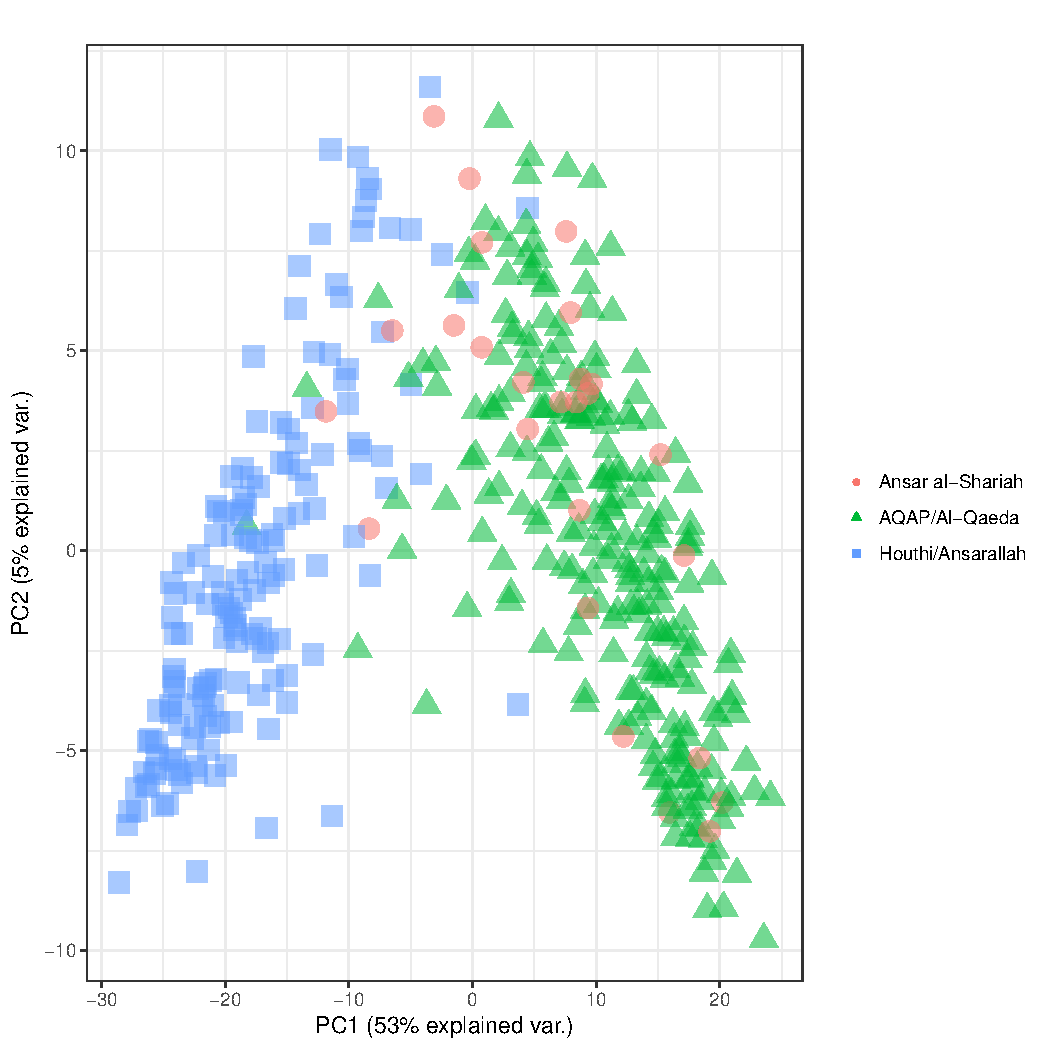
\includegraphics[width=5.00in]{./Pictures/pca_proximityRF.pdf}
\end{tabular}
\caption{PCA Visualization of Group Classification}
\label{fig:rf-pca}
\end{center}
 \end{figure}

%% Move to appendix b/c don't talk about SVM results in body of text.
%%The increasing uncertainty over time in the SVM classification is likewise ambiguous as the result largely derives from mispredicting AQAP-Houthi pairs.\footnote{Results are similar for a classification carried out on a subset of the corpus comprising just AQAP and Ansar al-Shariah stories.}

The clustering analysis is suggestive of convergence in reporting on activities of AQAP and Ansar al-Shariah. However, these methods do not adjudicate between competing explanations for the similarity. Potential reasons for the lack of differentiation include AQAP acting like Ansar al-Shariah; Ansar al-Shariah acting like AQAP; or the algorithms identifying shared features other than underlying behavioral similarity. Moreover, the news classification approach does not directly measure activity. In evaluating the style and coverage of third-party reporting, the results are sensitive to descriptive idiosyncrasies. For example, given the international salience of the al-Qaeda name, the news corpus likely contains over-attribution to AQAP. Similarly, under-attribution of Ansar al-Shariah activities can be introduced by journalists associating AQAP and Ansar al-Shariah.\footnote{Notably, 11 of the stories in the corpus carried language that blurred the distinction between AQAP and  Ansar al-Shariah. For example, an article from Xinhua News stated: \say{Al-Qaida in the Arabian Peninsula, also known locally as Ansar al-Sharia.}}  This may be a result of journalists including more contextual discussion as the security situation unraveled, thus dedicating article space to similar content. Alternately, the increased conflation of AQAP and Houthi stories may pick up a tendency of writers to frame AQAP mobilization using the rebellion frame that dominates coverage of Houthi activities.

\subsection*{Direction of Convergence}
\label{sec:direction-convergence}

A second approach to using text data as a window into opaque organizations leverages topic models applied to materials issued by the groups themselves. To adjudicate the possible direction of convergence in descriptions of AQAP and Ansar al-Shariah activity, I use the Structural Topic Model to summarize changes in latent topics within the corpus~\autocite{roberts2014stm}.  The model is well suited to addressing questions of convergence as it permits modeling group-level changes in attention over time by incorporating document-level information as a covariate related to topic prevalence. Existing work has applied the STM to a variety of corpora similarly comprised of short and moderate-length documents~\autocite{roberts2014structural}, such as open-ended surveys~\autocite{tingley2017rising}, social media messages~\autocite{bail2016cultural}, and deepweb forum posts~\autocite{munksgaard2016mixing}.

\subsection{Communique Analysis}
\label{sec:communiques}
To address the question of the direction of the apparent convergence of
AQAP and Ansar al-Shariah behavior, the following section presents
selected results from three Structural Topic Models estimated on AQAP
and al-Qaeda Central propaganda releases, showing a general
localizing trend in AQAP's self-presentation.\footnote{The Technical Appendix
  features information about text processing and a fuller
  characterization of the results.} The following analysis interprets rising prevalence of Yemen-specific topics and decreases in transnational and pan-jihadi topics as suggestive of an influential parochial base. The timing and content of any change in self-presentation can shed light on the question of whether the topic models reflect underlying ground truth: although communiques and speeches do not necessarily align perfectly with ground truth, finding that themes in AQAP self-presentation move along with the convergence in stories about AQAP and Ansar al-Shariah should bolster confidence that each technique is picking up a real change.

The analysis was conducted on a corpus of 875 documents released by al-Qaeda in the Arabian Peninsula from June 18, 2004 through September 18, 2016.\footnote{The corpus includes content from both the current--\textit{i.e.} post-2006--- AQAP and a predecessor organization of the same name that is occasionally referred to as al-Qaeda in Saudi Arabia.  AQAP is a direct successor to the Saudi Arabian-based \say{AQAP}, and the Yemen-based AQAP leadership actively sought to present the organizations as linked entities. Therefore, I allow the AQAP corpus to accommodate both the current Yemeni-based AQAP and the earlier Saudi-based \say{AQAP} as this permits examination of the impact of the upswing in drone casualties in 2009 and 2010.} The corpus consists of English translations of documents originally released in Arabic and, occasionally, the original text of English-language releases.\footnote{A very small portion of the
  documents, such as individual articles from \textit{Inspire Magazine}, were distributed in English.} These documents were collected and translated by the SITE Intelligence group, a private research organization that collects and translates jihadi media.\footnote{SITE Intelligence Group translations are advantageous for this project, as the company maintains near real-time coverage of prominent online distribution sites and has internal procedures to ensure consistent translation in style and tone.} As no official universal archive of AQAP's releases exists in the public domain,  the corpus is necessarily a sample of the releases. However, as the SITE Intelligence Group is an internationally-focused monitoring
  organization, any systematic selection effects should bias the results against finding increased local self-presentation because bias could be expected to prioritize documents intended for an international audience which should then carry an internationalist message.
  
Official releases are an attractive source of information about changing organizational priorities because, within certain ideological constraints, these documents
provide a forum on which an organization can choose how to
frame their self-presentation. As well, the technological environment makes propaganda documents appealing in this context: since 2011, online platforms have been a \say{major means of communication} within
Yemen~\autocite[33]{carapico2014yemen}. This implies that media distributed online can be consumed by domestic as well as international audiences. The two-level audience can be expected to discourage AQAP from strategically differentiating their online
signaling from their local self-presentation. Readers may worry that even if online platforms are important for communication in the country, Yemen's relatively low internet penetration rate may imply that AQAP's online propaganda is not intended for a domestic audience. If this the case, it should likewise bias the results against findings in support of the bottom-up localizing hypothesis.\footnote{As well, one may be concerned that a strategic actor could use in-person networks to signal which documents are intended for local versus international audiences. However, the difficult information and security environment in Yemen makes it risky to rely on a bifurcated media strategy.} 
The first model addresses the question of direction of convergence in third-party reporting about the activities
of AQAP and Ansar al-Shariah. The outcome predicted by the bottom-up theory of organizational change
expects that an influx of fighters was followed by AQAP adopting a
more local, Yemeni-centric, self-presentation. A second model addresses the counterfactual that regional  and global developments may account for changes in AQAP messaging, independent of any changes in membership base. To account for the possibility that observed shifts in messaging were driven by top-down directions from al-Qaeda leadership or general trends in the jihadi environment, the model contrast the rhetoric of AQAP with that
featured in an additional 500 documents released by as-Sahab, a media
production house closely associated with al-Qaeda's senior leadership.  Finally, a model that evaluates the differences between AQAP's presentation of their \say{Ansar al-Shariah} and the main AQAP branding can be found in the Technical Appendix. This model verifies the operating assumption AQAP's propagandists sought to depict Ansar al-Shariah as the more locally-involved Sunni militant group.

\underline{Model: Evolution of AQAP Messaging}\\

The first model characterizes the evolution of AQAP messaging across the 875 documents in the corpus in order to evaluate trends in the
thematic content of AQAP's messaging.  The bottom-up transformation
theory described above predicts that an influx of local
recruits should encourage AQAP to adopt increasingly local
priorities, and thus that convergence in third-party media coverage of
AQAP and Ansar al-Shariah should be driven by changes in AQAP.  If, as
argued above, organizational messaging tracks true organizational
priorities, changes in AQAP's focus should manifest in the topic model
identifying an increased prevalence of themes relating to domestic fissures, such as the Houthi-Sunni civil war, and a decline of transnational themes. 

Although general trends alone are unable to directly test the predictions of the bottom-up transformation theory, relative differences in the proportions of themes can indicate the general plausibility of the argument. In the
case of Yemen, the theory predicts that increased access to local
recruits should drive AQAP to adopt an increasingly localized
agenda. If AQAP is increasing attention to domestic considerations and themes, the localizing trend suggests that changes in AQAP are driving the difficulty in classifying AQAP and Ansar al-Shariah's activity.\footnote{Analysis of the differing ways in which AQAP presents itself in communiques released under the AQAP and Ansar al-Shariah "brands" can be found in the Technical Appendix.}

Attention within the AQAP corpus is modeled via an 18-topic structural
topic model.\footnote{For discussion of model specification, see the accompanying Technical Appendix.} The topics are presented in Figure~\ref{fig:topicSumsED}, clustered into four thematic groupings: locally-focused war reports, discussions about and threats of clandestine operations, topics promoting transnational jihadi sentiments and goals, and jihadi-associated descriptors. Within each cluster, topics are summarized by their FREX words, which are words or tokens that are associated with the topic but relatively unlikely elsewhere in the corpus. Figure~\ref{fig:EDModelTopicProportions} shows what proportion of the entire corpus of communiques is expected to be assigned to each of the fifteen substantively interesting topics.\footnote{The three remaining topics relate to the construction of the documents themselves, and are less interesting as a reflection of AQAP's self-presentation. These topics relate to videography, habitual sign-off terms, and transcript production.}  As the figure indicates, when the entire corpus is taken together without any disaggregation by document release date, the two most common topics are relate to the Houthi militias and terms that describe local targets and operations. From there, a number of topics that associate words around ideological and tactical themes are each expected to feature in about 10\% of the total documents.

\begin{figure*}
\begin{center}
  \caption{Groupings of Substantive Topics in General Trends Model}
  \label{fig:topicSumsED}
  \begin{tabular}{cc}
 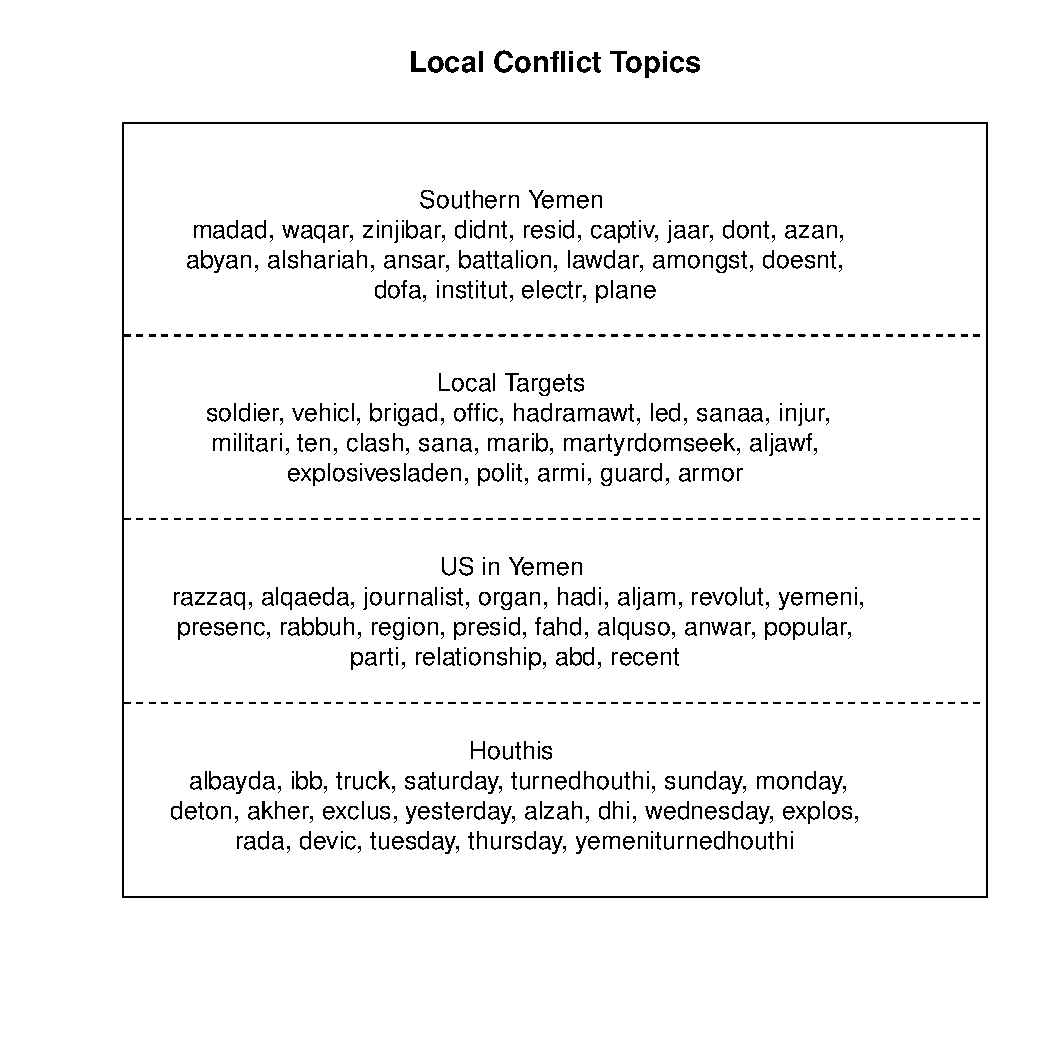
\includegraphics[width=.49\columnwidth]{./Pictures/dayModel_UT70_cluster1.pdf}&  
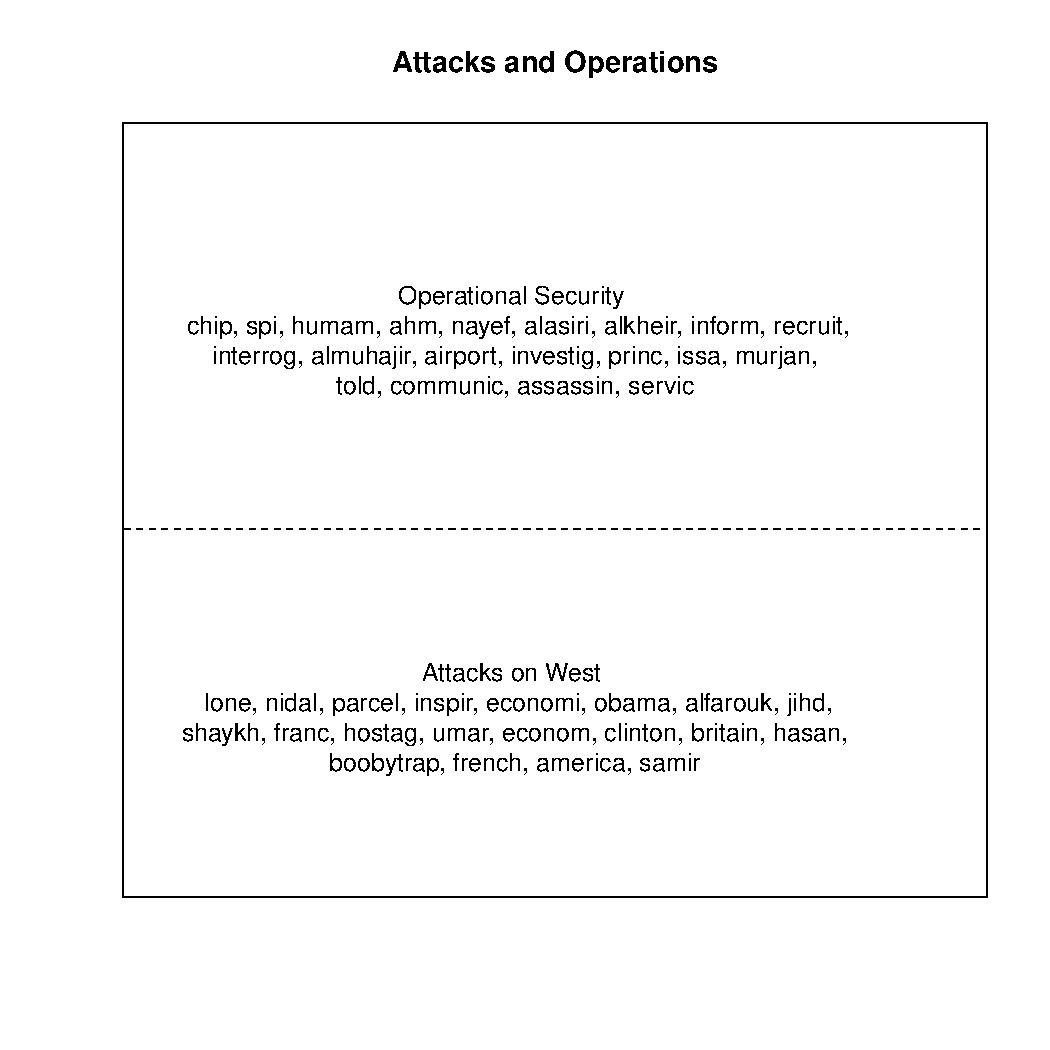
\includegraphics[width=.49\columnwidth]{./Pictures/dayModel_UT70_cluster2.pdf}\\
\vspace{-1.00cm}
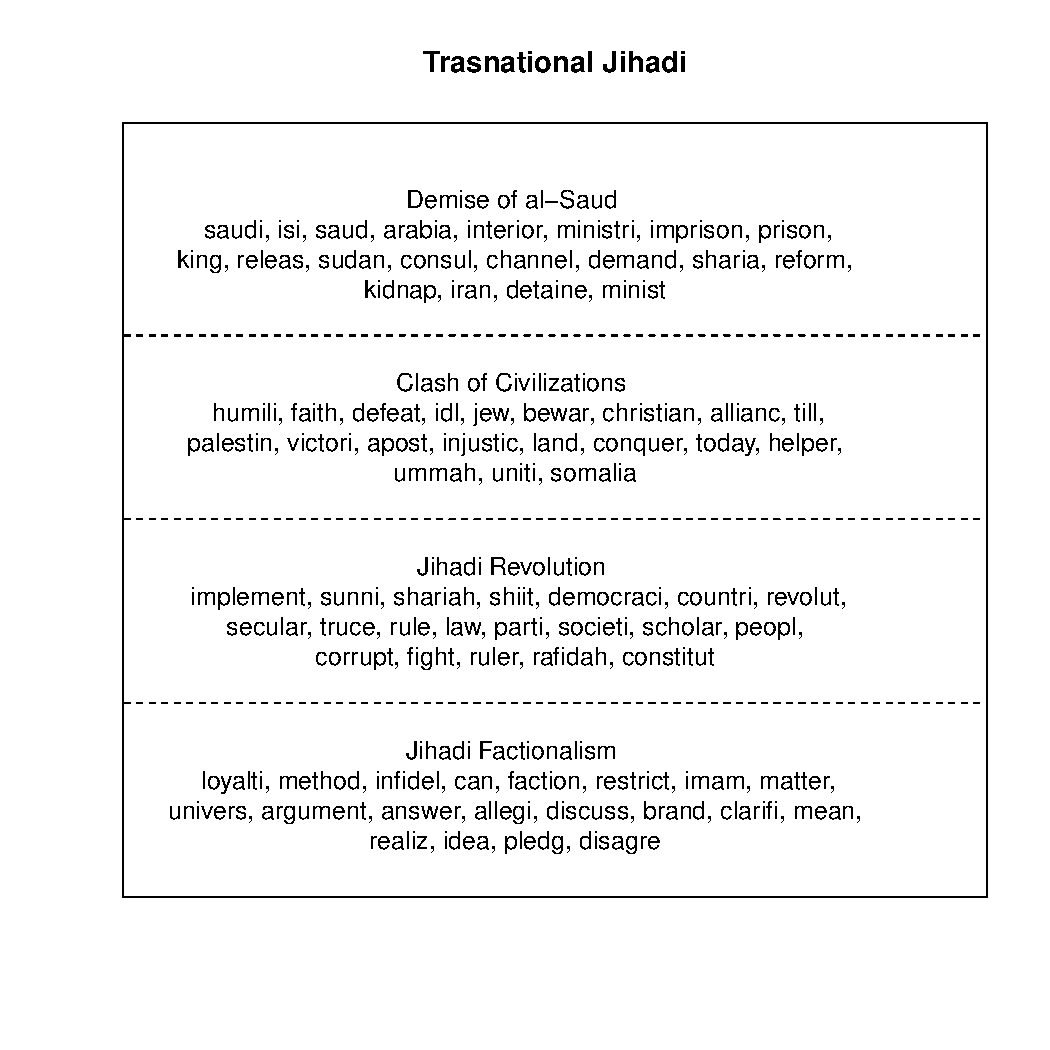
\includegraphics[width=.49\columnwidth]{./Pictures/dayModel_UT70_cluster3.pdf}&  
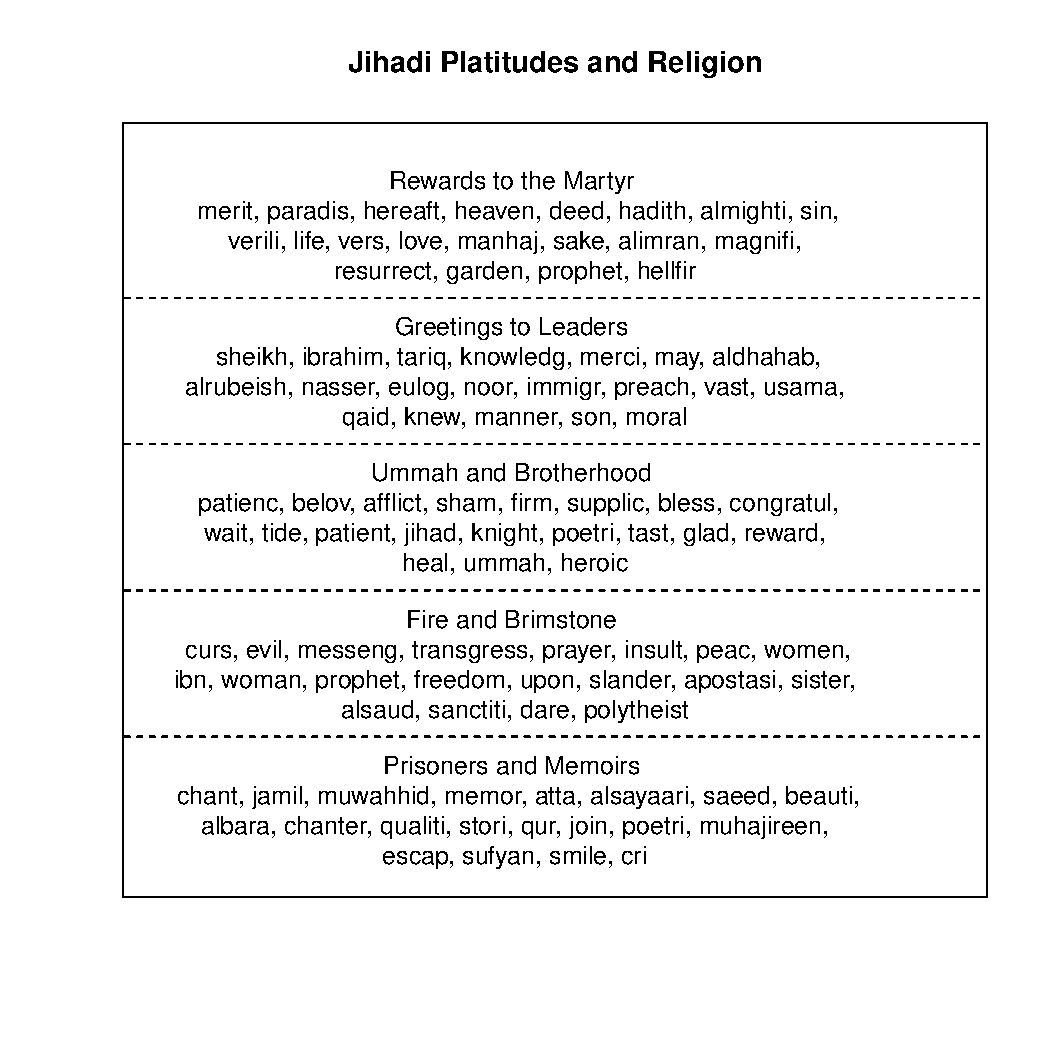
\includegraphics[width=.49\columnwidth]{./Pictures/dayModel_UT70_cluster4.pdf} \\
  \end{tabular}
\end{center}
  \end{figure*}

\begin{figure*}
  \begin{center}
  \begin{tabular}{c}
    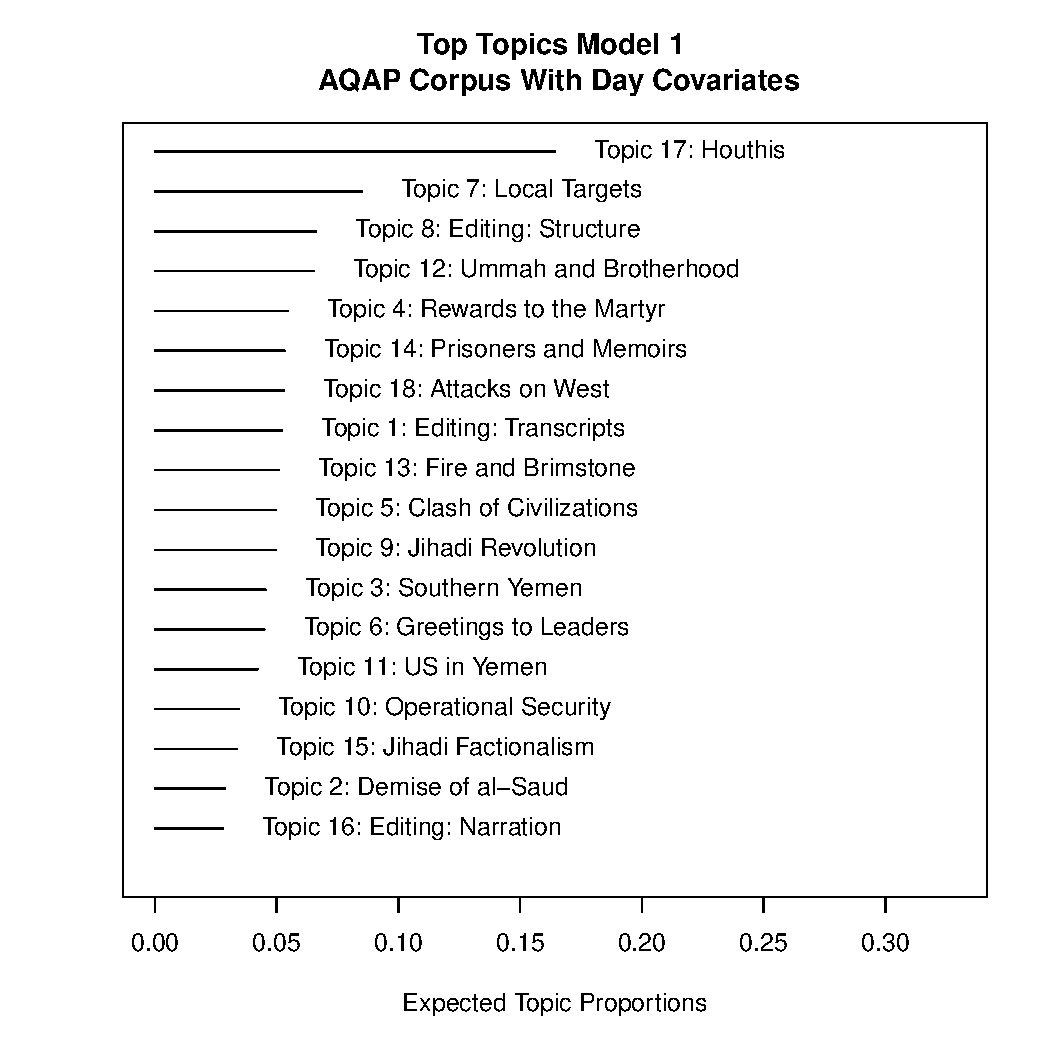
\includegraphics[width=4.00in]{./Pictures/topicProportions_UT70EDModel.pdf}\\
  \end{tabular}
  \caption{Estimated Topic Proportions in al-Qaeda in the Arabian
    Peninsula Corpus}
  \label{fig:EDModelTopicProportions}
\end{center}
\end{figure*}

The relative frequency of topics specifically about Yemen provide the
first place to look for evidence of a local trend in AQAP's messaging. As several of the thematic clusters identified by the model relate to various facets of AQAP's activities in Yemen---including discussion of Houthi militants, activities in Southern Yemen, castigation of the Yemeni government, and descriptions of local operations--- combining the estimated prevalence of each Yemen-centric topic gives an easily-visualized overview of the changing salience of local concerns in AQAP propaganda output. Figure~\ref{fig:l-t-clusters} depicts the expected document-level topic
proportion for the \say{Local Conflict} cluster. The cluster is characterized by words that refer to specific local operations, geography, and political jurisdictions.  Indeed, documents representative of this topic are often battlefield communiques issued to claim local
territorial control. Even the most transnational of the topics, the
\say{US in Yemen} topic, emphasizes political events in the country.
Thus, document space dedicated to each of the \say{Local Conflict}
topics reflects a prioritization of domestic Yemeni issues over
transnational themes. Furthermore, a localizing trend is underscored by looking at changes in the expected prevalence of the four topics that speak to a transnational jihadi sentiment. These topics refer to regional power centers, notably the government and security apparatus of Saudi Arabia, and social concerns that are typical of the transnational jihadi movement. Taken together, the prevalence of these four topics begins to decline from a peak in late 2012, as AQAP's propaganda becomes increasingly focus on the local Yemeni civil war.\footnote{Readers might be concerned that the inverse relationships between topic proportion allocated to the \say{transnational} and \say{local conflicts} are simply mechanical. Although the total prevalence assigned to all topics in the model does sum to one, and thus increased attention to one topic necessarily means less attention to others, the \say{transnational} and \say{local
conflicts} clusters never exceed an expected topic percentage of 75\%
of any given document. Moreover, the mean expected topic proportions dedicated to the two topics is 45\%. Thus, the two topics could co-exist if desired by AQAP's propagandists.}

\begin{figure*}
\begin{center}
\begin{tabular}{c}
  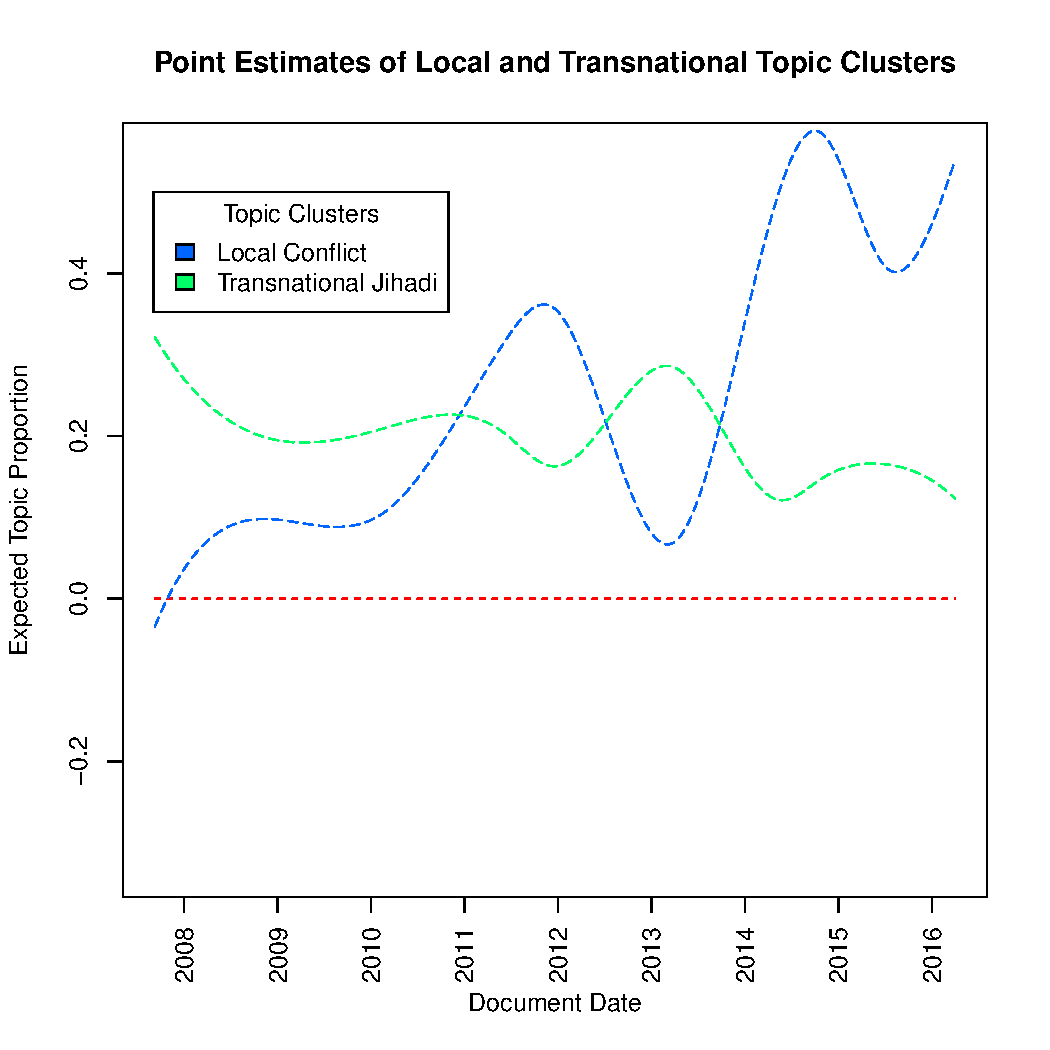
\includegraphics[width=5.00in]{./Pictures/localtranscluster.pdf}\\
\end{tabular}
\caption{Changes over time to attention dedicated to local and transnational themes }
\label{fig:l-t-clusters}
\end{center}
 \end{figure*}

\subsection{Comparison to Central al-Qaeda Messaging}
\label{sec:STM3}
Thus far, the analysis has suggested that local observers generally
characterized AQAP and Ansar al-Shariah using similar terminology and
framing, and despite investment in Ansar al-Shariah as the local face of the movement, AQAP's communiques become progressively
more local in theme.  Although these results are generally
consistent with the theory's expectation that an influx
of local fighters generated internal pressure on AQAP to focus on
local issues, an alternate explanation could point to broader forces
among the transnational jihadi community. In particular, 2011, the year of
the Yemeni Revolution, also saw a series of shockwaves through the
jihadi world after Usama bin Laden was killed on May 2, 2011. His second in command,
Ayman al-Zawahiri, subsequently assumed leadership of the global
al-Qaeda network. In September of that year, an American drone strike
killed Anwar al-Awlaki, an American-Yemeni cleric who had been a
strident internationalist face for AQAP.

The deaths of bin Laden and Awlaki, and Ayman al-Zawahiri's subsequent
ascendance to the leadership of al-Qaeda, are challenging for the theory
developed above. Al-Zawahiri has long been associated with an
internal al-Qaeda faction that prioritizes focusing on implementing
country-specific social and political revolutions in the home
countries of al-Qaeda's operatives, rather than engaging in
civilizational struggle against the American-lead global
system~\autocite[147]{miller2015audacious}. Correspondingly, Awlaki was
instrumental in AQAP's efforts to radicalize and mobilize fighters
internationally, particularly from the West.

Thus, one possible counter-narrative to the bottom-up transformation
argument maintains that the change in al-Qaeda's leadership may have triggered a wider ideological shift that filtered to local branches and that Awlaki's death amplified
the effect in Yemen. Indeed, if AQAP was following the lead of al-Qaeda Central after 2011, changes in AQAP's self-presentation would not be informative about the grassroots transformation theory.

To differentiate a local change in Yemeni rhetoric from changes prompted by a top-down al-Qaeda strategy, this section presents selected results from a structural topic model that estimated topic prevalence in a corpus of propaganda released by AQAP and as-Sahab, al-Qaeda's central media wing.  AQAP's changing rhetorical style is presented alongside that of as-Sahab to establish that observed changes in AQAP rhetoric are not driven by an underlying pan-jihadi trend. This model, Model Two, identified themes in a corpus of 1375 documents, of which 875 were AQAP communiques and 500 were  releases from as-Sahab. The model predicted topic prevalence as a function of time interacted with whether the document was authored by AQAP or as-Sahab.\footnote{Time is included in this model as a linear function for computational tractability.}

The patterns are generally intuitive: overall AQAP is more likely to talk about
Yemen-related topics while topics that discuss other battlegrounds and
targets for revolution are more associated with as-Sahab.\footnote{A
  full analysis is discussed in the Technical Appendix} However, the
divergence in thematic prevalence of pan-jihadi topics between
releases issued by as-Sahab and AQAP indicate that AQAP's increasing
Yemen focus was not indicative of a localizing turn lead or directed
by al-Qaeda Central, via their as-Sahab mouthpiece. Two such themes are highlighted below. The two highlighted themes were chosen for their popularity among globally-minded jihadis. The first is characterized by an explicitly transnational list of FREX words: it features countries with active jihadi battlegrounds as well as references to what jihadis perceive as an American-Israeli alliance against Muslims around the world. The second topic is a relatively abstract transnational theme that attempts to mobilize jihadi supporters by referencing vulnerable demographics of Muslims, such as women and children, experiencing hardship and travails.

Figure~\ref{fig:crusaders} highlights two topic outcomes from the model.  The first topic is analogous to both of the \say{Clash of Civilizations} topics above, here titled  \say{Crusaders and Zionists.}\footnote{As a different model, the topics are unique to this model although generally similar to the themes from Models One and Two.}  This topic is notable for having a strong transnational jihadi focus; exactly the type of subject that AQAP should cease to discuss if their domestic recruitment is
driving a local focus. Indeed we see that although al-Qaeda Central's
rhetoric does increasingly feature this topic, AQAP becomes
progressively less and less inclined to use words associated with the
topic. Interestingly, AQAP's move away from the ``Crusaders and
Zionists'' topic occurs even though AQAP documents were originally more likely to feature the topic than were as-Sahab documents.

Similarly, after 2011, as-Sahab documents become more likely to
discuss a topic addressing alleged injustices against vulnerable
populations such as women and children. The topic, which I name ``Defending
the Weak,'' expresses indignation about alleged crimes against Muslim
women and children and is a pervasive theme of transnational jihadi
rhetoric. Throughout the time period covered by the corpus, the topic
becomes less common in AQAP documents and more prevalent in as-Sahab releases. 

\begin{figure*}
\begin{center}
  \caption{AQAP and as-Sahab Divergence}
  \label{fig:crusaders}
  \begin{tabular}{cc}
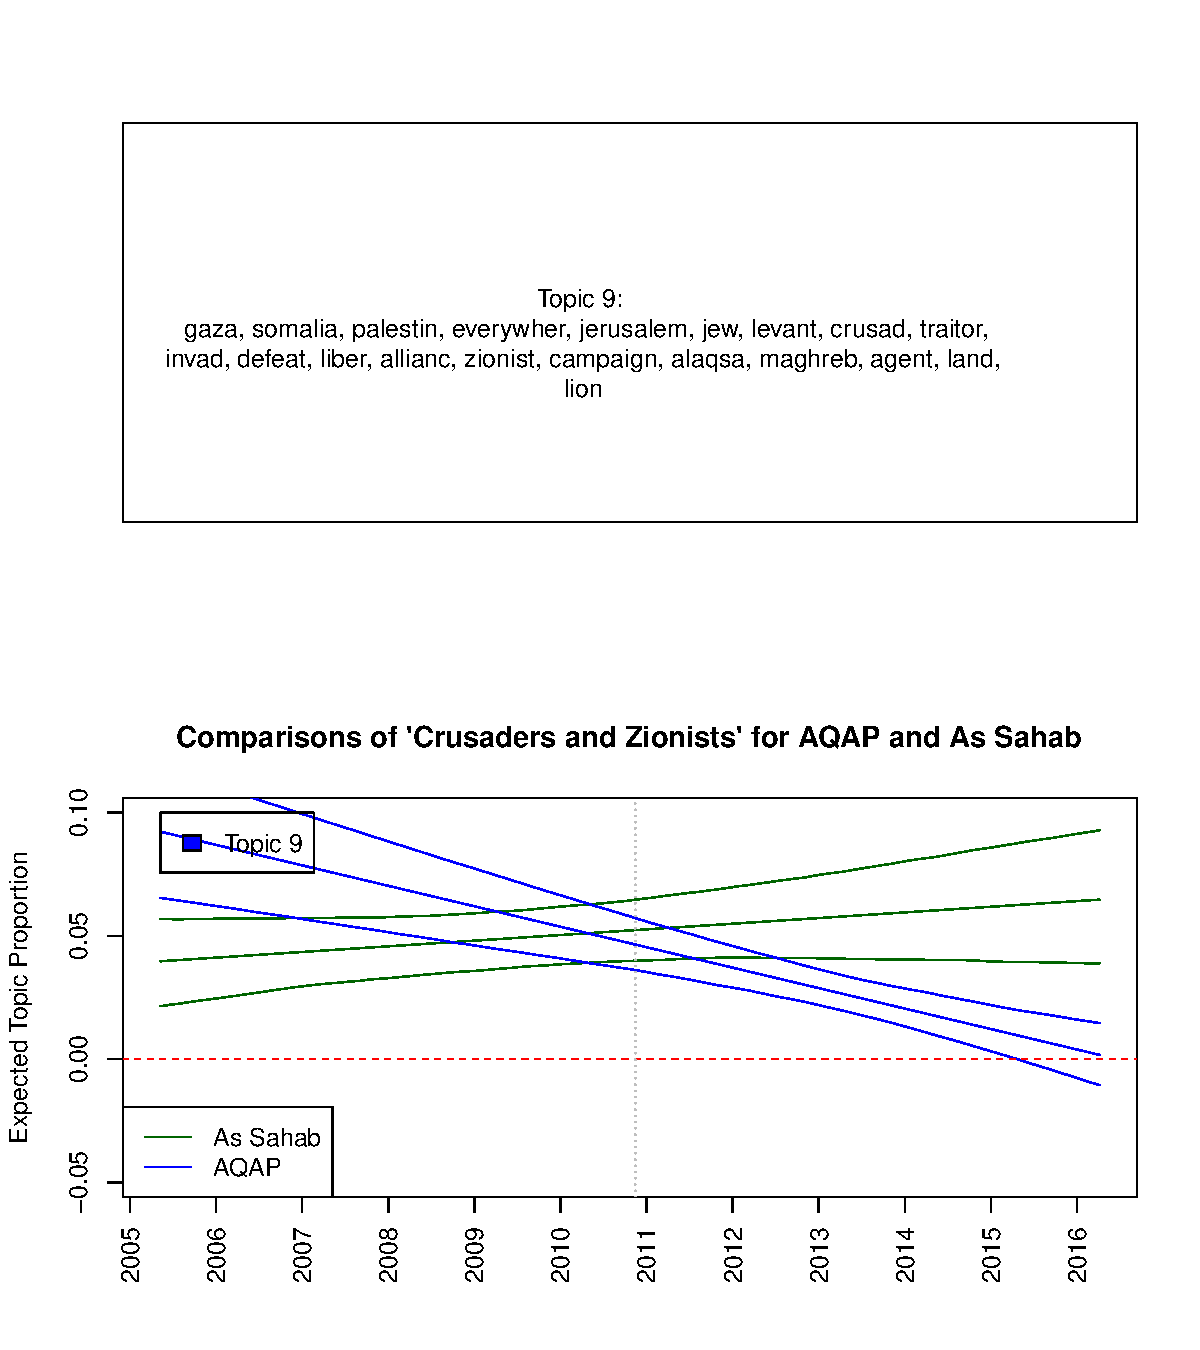
\includegraphics[width=.45\columnwidth]{./Pictures/34TopicsComparisonCrusaderZionists2.pdf}&
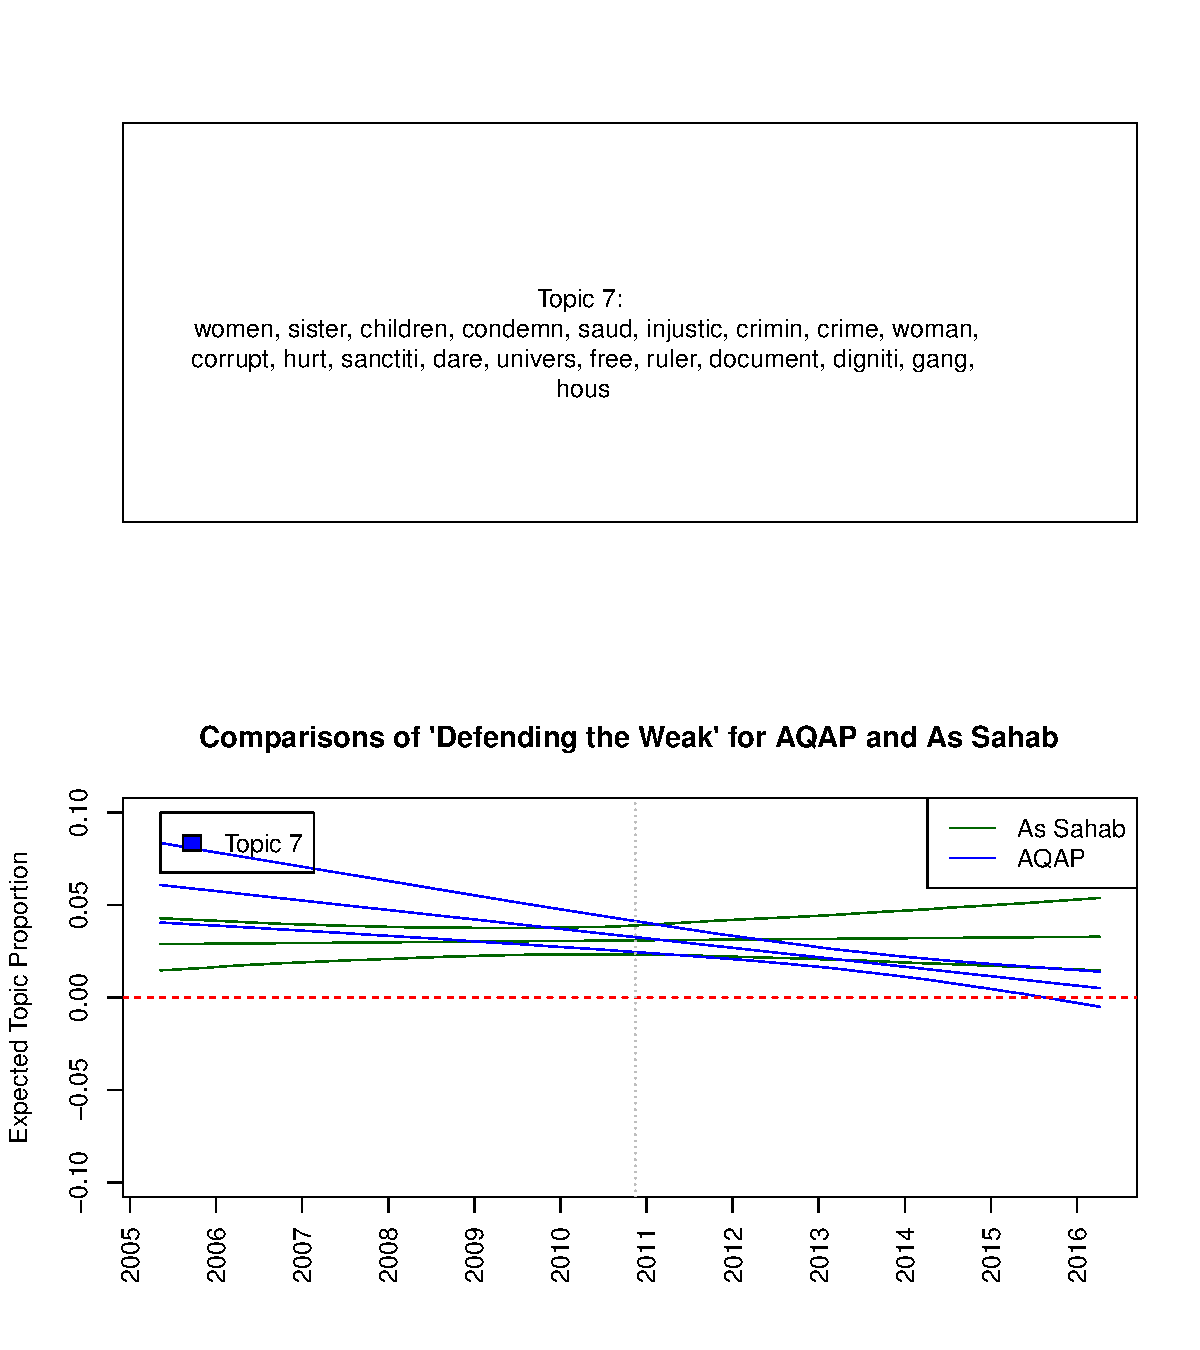
\includegraphics[width=.45\columnwidth]{./Pictures/34DefenseofWomen.pdf}\\
  \end{tabular}
\end{center}
 \end{figure*}
